\documentclass[a4paper,12pt,twoside,openright,titlepage]{book}

%Additional packages
\usepackage[ascii]{inputenc}
\usepackage[T1]{fontenc}
\usepackage[dutch,english]{babel}
\usepackage{syntonly}
\usepackage[official]{eurosym}
%\usepackage[graphicx]
\usepackage{graphicx}
\graphicspath{ {./images/} }
\usepackage{float}
\usepackage{xurl}
\usepackage{hyperref}
\hypersetup{colorlinks=true, linkcolor=blue, citecolor=blue, filecolor=blue, urlcolor=blue, pdftitle=, pdfauthor=, pdfsubject=, pdfkeywords=}
\usepackage{tabularx}
\usepackage{scrextend}
\addtokomafont{labelinglabel}{\sffamily}
\usepackage{listings}
\usepackage{adjustbox}

%define inch
\usepackage{mathpazo,amsmath}
\def\inch#1{#1''}

% Turn on indexing
\usepackage{imakeidx}
\makeindex[intoc]

% Define colors
\usepackage{color}
\definecolor{ashgrey}{rgb}{0.7, 0.75, 0.71}

% Listing style
\lstset{
  backgroundcolor=\color{ashgrey},   % choose the background color; you must add \usepackage{color} or \usepackage{xcolor}; should come as last argument
  basicstyle=\footnotesize,        % the size of the fonts that are used for the code
  breakatwhitespace=false,         % sets if automatic breaks should only happen at whitespace
  breaklines=true,                 % sets automatic line breaking
  extendedchars=true,              % lets you use non-ASCII characters; for 8-bits encodings only, does not work with UTF-8
  frame=single,	                   % adds a frame around the code
  keepspaces=true,                 % keeps spaces in text, useful for keeping indentation of code (possibly needs columns=flexible)
  rulecolor=\color{black},         % if not set, the frame-color may be changed on line-breaks within not-black text (e.g. comments (green here))
  showspaces=false,                % show spaces everywhere adding particular underscores; it overrides 'showstringspaces'
}

% Uncomment for production
% \syntaxonly

% Style
\pagestyle{headings}

%%%%%%%%%%%%%%%%%%
% Begin document %
%%%%%%%%%%%%%%%%%%

% Define document
\author{D. Leeuw}
\title{Security: Webservers}
\date{\today\\v.0.3.0}

\begin{document}
\selectlanguage{dutch}

\maketitle

\copyright\ 2021 Dennis Leeuw\\

\begin{figure}[H]

\includegraphics[width=0.3\textwidth]{CC-BY-SA-NC.png}
\end{figure}

\bigskip

Dit werk is uitgegeven onder de Creative Commons BY-NC-SA Licentie en laat anderen toe het werk te kopi\"eren, distribueren, vertonen, op te voeren, en om afgeleid materiaal te maken, zolang de auteurs en uitgever worden vermeld als maker van het werk, het werk niet commercieel gebruikt wordt en afgeleide werken onder identieke voorwaarden worden verspreid.


%%%%%%%%%%%%%%%%%%%
%%% Introductie %%%
%%%%%%%%%%%%%%%%%%%

\frontmatter
\chapter{Over dit Document}
Dit boek behandelt security van webservers.

\section*{Versienummering}
Het versienummer van elk document bestaat uit drie nummers gescheiden door een punt. Het eerste nummer is het major-versie nummer, het tweede nummer het minor-versienummer en de laatste is de nummering voor bug-fixes.\par
Om met de laatste te beginnen als er in het document slechts verbeteringen zijn aangebracht die te maken hebben met type-fouten, websites die niet meer beschikbaar zijn, of kleine foutjes in de opdrachten dan zal dit nummer opgehoogd worden. Als docent of student hoef je je boek niet te vervangen. Het is wel handig om de wijzigingen bij te houden.\par
Als er flink is geschreven aan het document dan zal het minor-nummer opgehoogd worden, dit betekent dat er bijvoorbeeld plaatjes zijn vervangen, geplaatst of weggehaald, maar ook dat paragrafen zijn herschreven, verwijderd of toegevoegd, zonder dat de daadwerkelijk context is veranderd. Een nieuw cohort wordt aangeraden om met deze nieuwe versie te beginnen, bestaande cohorten kunnen doorwerken met het boek dat ze al hebben.\par
Als het major-nummer wijzigt dan betekent dat dat de inhoud van het boek substantieel is gewijzigd om bijvoorbeeld te voldoen aan een nieuw kwalificatiedossier voor het onderwijs. Een nieuw major-nummer betekent bijna altijd voor het onderwijs dat men in het nieuwe schooljaar met deze nieuwe versie aan de slag zou moeten gaan. Voorgaande versies van het document zullen nog tot het einde een schooljaar onderhouden worden, maar daarna niet meer.

\section*{Document ontwikkeling}
Het doel is door middel van open documentatie een document aan te bieden aan zowel studenten als docenten, zonder dat hier hoge kosten aan verbonden zijn en met de gedachte dat we samen meer weten dan alleen. Door samen te werken kunnen we meer bereiken.\par
Bijdragen aan dit document worden dan ook met alle liefde ontvangen. Let u er wel op dat materiaal dat u bijdraagt onder de CC BY-NC-SA licentie vrijgegeven mag worden, dus alleen origineel materiaal of materiaal dat al vrijgegeven is onder deze licentie.

\begin{flushleft}
\begin{table}[h!]
\centering
	\begin{tabularx}{\textwidth}{ |p{0.1\linewidth}|p{0.3\linewidth}|p{0.5\linewidth}| }
\hline
	Versie &
	Auteurs &
	Wijzigingen\\
\hline
	0.3.0 &
	Dennis Leeuw &
		Extra uitleg bij webserver encryptie (TLS) als achtergrond informatie\\
\hline
	0.2.0 &
	Dennis Leeuw &
	Non-disclosure hoofdstuk gesplitst in client-side (informatie verzamelen) en server-side (informatie vrijgeven)\\
\hline
	0.1.0 &
	Dennis Leeuw &
	Twee nieuwe hoofdstukken: Non-disclosure, Webserver encryption en titel wijziging naar Security: Webserver\\
\hline
	0.0.2 - 0.0.3 &
	Dennis Leeuw &
	Verwerking opmerkingen Monique Petra en verdere uitbreiding\\
\hline
	0.0.1 &
	Dennis Leeuw &
	Ontwikkelversie\\
\hline
\hline
\end{tabularx}
\caption{Document wijzigingen}
\label{table:1}
\end{table}
\end{flushleft}



%%%%%%%%%%%%%%%%%
%%% De inhoud %%%
%%%%%%%%%%%%%%%%%
\tableofcontents

\mainmatter

\chapter{Een veilige webserver}
We bouwen in dit document een beveiligde webserver op. Omdat het een server is gaan we er vanuit dat je een server operating system gebruikt. Voor Windows is dat dan Windows Server. Voor Linux maakt het niet zo veel uit, hoewel we er wel vanuit gaan dat er geen grafische interface ge\"installeerd is, dus dat je alles op de command line doet in Linux.

Dit document behandelt niet alle facetten van webserver security. Het is bedoeld als inleiding en om je een idee te geven wat er allemaal komt kijken bij het beveiligen van websites. Uitgebreidere informatie is te vinden op het het Internet, vooral de website van Mozilla \url{https://www.mozilla.org} bevat veel goede documentatie.

\section{Client side information}
Via de webbrowser haal je data op vanaf een webserver. Je browser zorgt ervoor dat de opgehaalde data wordt afgebeeld op je scherm zoals het door de ontwerpers van de site bedoeld is. Om deze uitwisseling van data mogelijk te maken zijn er een aantal zaken noodzakelijk:
\begin{itemize}
\item Een taal waarmee browser en server elkaar verstaan: het netwerk protocol HTTP
\item Een taal om duidelijk te maken hoe de data weergegeven moet worden: de opmaak taal HTML en CSS
\item De uit te wisselen data
\end{itemize}

Om met het laatste te beginnen, de data, dat is alle informatie die je via het web zou kunnen uitwisselen, zoals tekst, plaatjes, video en muziek. Al deze data kan in een bepaalde opmaak (layout) worden aangeboden.

HTML (HyperText Markup Language) en CSS (Cascaded Style Sheets) zijn de onderdelen die bepalen hoe de data op het scherm weergegeven moeten worden, we noemen ze dan ook wel opmaaktalen of markup languages in het Engels. HTML beschrijft de elementen in een document, dus HTML beschrijft of iets een paragraaf is, of een titel van een document en CSS vertelt daarna hoe die paragraaf of titel weergegeven moet worden, lettertype, grootte, dik of niet dik gedrukt.

Tot slot moet de data met alle opmaak, plaatjes, etc. over het netwerk getransporteerd worden en dat gebeurt door HTTP, het HyperText Transfer Protocol. HTTP zorgt voor het transport van data en bij dat transport horen ook headers die meer zeggen over de data, het is de zogenaamde META-data, dus data die iets vertelt over de data. Zo heeft een web-pagina een header die Content-Type heet en die zegt dat de aangeboden data text/html is, het is dus platte tekst, geen binaire data, en de opmaak is in html. Een plaatje kan een header hebben Content-Type: image/png. Elk element van een website heeft zo zijn eigen META-data (headers). De headers kunnen ook gebruikt worden om bepaalde security maatregelen door te geven. Dit kan van de client naar de server en van de server naar de client.

\section{Website debugging}
De moderne browsers, Firefox, Chrome, Edge, Opera, etc. hebben een functie om ontwikkelaars, maar ook nieuwsgierigen, te laten weten wat ze achter de schermen allemaal gedaan hebben om de pagina op het scherm te krijgen. Veel van deze informatie is alleen handig voor website ontwikkelaars maar sommige informatie is ook handig voor het controleren van de veiligheid van websites. Bijna alle browsers gebruiken de F12-toets om deze extra functie op te roepen. Binnen Edge wordt het de Developer Tools genoemd, bij Firefox vind je het in het menu onder Web Developer en Chrome noemt het natuurlijk ook Developer tools, want Edge gebruikt Google Chrome als engine.

\subsection{Microsoft Edge}

Ga naar de pagina of website die je wil analyseren en druk op F12, je krijgt een figuur te zien zoals in figuur \ref{fig:EdgeF12}.
\begin{figure}[h]
	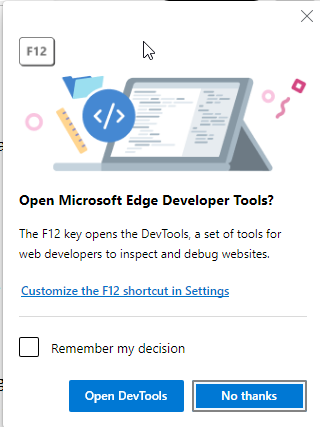
\includegraphics[]{edge_F12.png}
	\caption{F12 Debugging functie Microsoft Edge}
	\label{fig:EdgeF12}
\end{figure}
Klik op Open DevTools (eventueel kan je aanvinken dat Microsoft deze keuze moet onthouden).

Daarna kom in de Developer Tools terecht. Je krijgt dan naast de website die je bezoekt een uitgebreidde debugging tool zoals weergegeven in figuur \ref{fig:EdgeDebugger}.
\begin{figure}[h]
	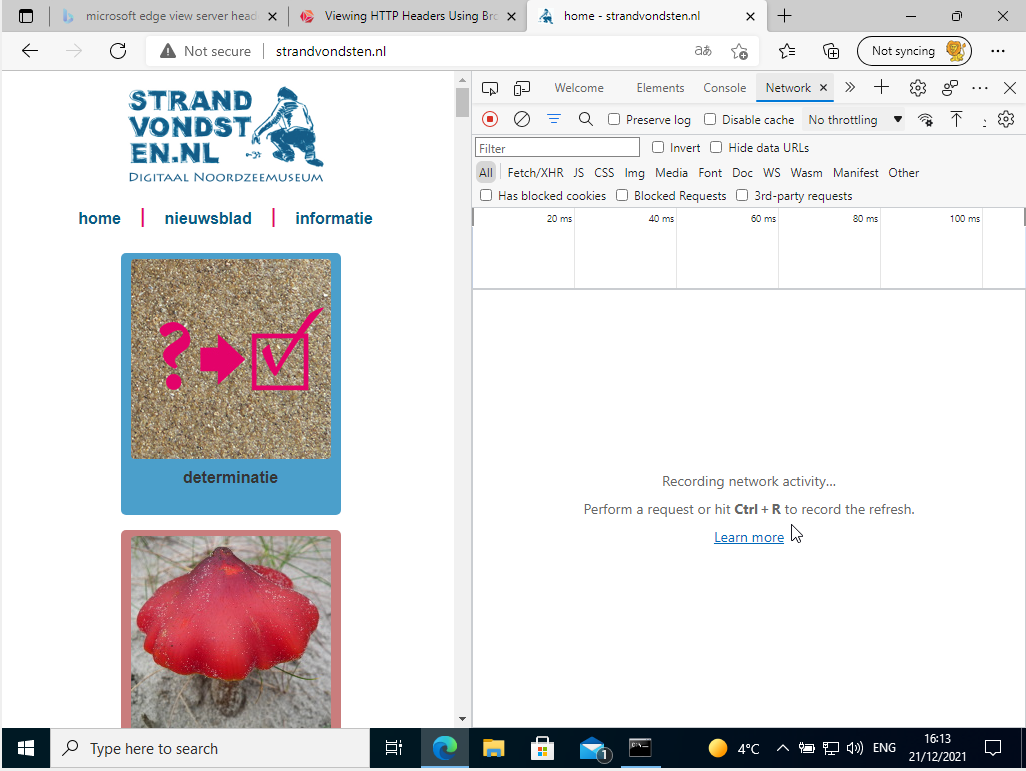
\includegraphics[width=0.9\linewidth]{Edge_Debugger.png}
	\caption{Microsoft Edge Developer Tools}
	\label{fig:EdgeDebugger}
\end{figure}


Selecteer in de balk met Welcome de Network tab en reload de pagina (aan de linker kant). Het scherm zal er dan ongeveer zo uit zien als in figuur \ref{fig:EdgeHeaders}.
\begin{figure}[h]
	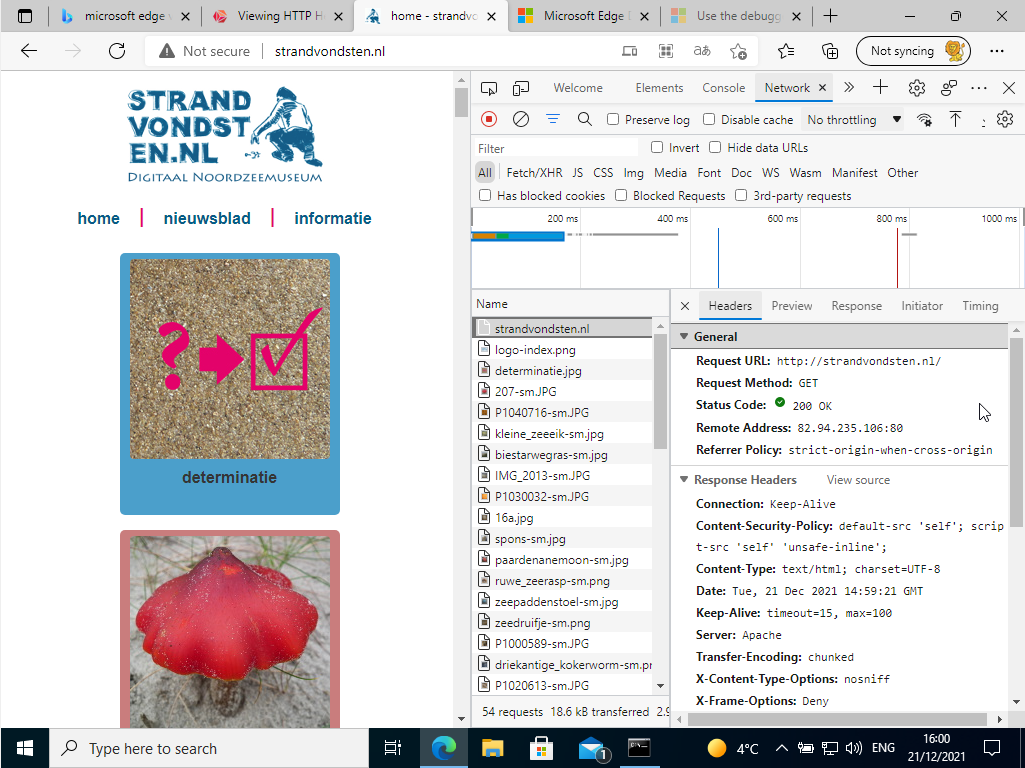
\includegraphics[width=0.9\linewidth]{Edge_Headers.png}
	\caption{Weergave van HTTP headers in Microsoft Edge}
	\label{fig:EdgeHeaders}
\end{figure}
Klik op het Headers tabblad en scroll aan de rechter onderkant helemaal omhoog en selecteer het bovenste element (in het voorbeeld: strandvondsten.nl), je ziet dan de headers die van de server terug zijn gekomen. Het zijn deze headers die van belang zijn in de rest van het document en die je op deze manier kan controleren.


\chapter{Non-disclosure}
\section{Apache}\index{Apache}
\subsection{Version disclosures}\index{Apache!Version disclosure}
In de httpd.conf set
\begin{lstlisting}
ServerTokens Prod
\end{lstlisting}
Dit voorkomt dat Apache zijn versie nummer meegeeft in de response header. De default voor deze parameter is 'Full'

Een andere waarde die handig is om te zetten in httpd.conf is:
\begin{lstlisting}
ServerSignature Off
\end{lstlisting}
met deze setting zal Apache ook de versie niet weergeven op de door de server gegenereerde pagina's zoals bijvoorbeeld de error pagina's.

Als je wil voorkomen dat bekend wordt dat de server een Apache server is dan met je gebruik maken van modSecurity, daarmee kan je ook voorkomen dat de server zich meldt als Apache server.

\section{NGINX}\index{NGINX}
\subsection{Version disclosures}\index{NGINX!Version disclosure}
In het nginx.conf bestand zet:
\begin{lstlisting}
server_tokens off;
\end{lstlisting}
zodat NGINX zijn versie nummer niet weergeeft in de response headers.

\section{IIS}
\subsection{Version disclosures}\index{IIS!Version disclosure}\index{Version disclosure!IIS}
Om te zorgen dat IIS niet aan de hele wereld gaat lopen vertellen welke versie het is en welke ASP.NET versie het gebruikt doorloop je de volgende stappen:
\begin{enumerate}
\item Open "Internet Information Services (IIS) Manager".
\item Als het voor alle websites moet gelden (globaal), klik: "Select IIS node"
\item Open de "Configuration Editor"
\begin{description}
\item[x-aspnet-version] Voor het verwijderen van de x-aspnet-version header ga naar system.web, httpRuntime, enableVersionHeader en zet het naar 'false'
\item[server] Voor het verwijderen van de server header ga naar system.webServer, security, requestFiltering, removeServerHeader en zet het naar 'true'
\end{description}
\item Klik op "HTTP Response Headers"
\item Selecteer "X-Powered-By" header en klik op 'Remove'
\end{enumerate}

Om te voorkomen dat Microsoft de API versie vrij geeft zet als laatste:
\begin{enumerate}
	\item Open de registry editor
	\item ga naar:
		\begin{lstlisting}
Computer\HKEY_LOCAL_MACHINE\SYSTEM\CurentControlSet\Services\HTTP\Parameters
		\end{lstlisting}
	\item zet de DisableServerHeader (REG\_DWORD) registry key van 0 naar 1
\end{enumerate}

\subsection{Methods}
De meeste webserver hoeven niet alle commando's (methods) te ondersteunen. GET, HEAD en POST zijn over het algemeen voldoende. Het uitschakelen van de overige methods OPTIONS, PUT, DELETE, TRACE, CONNECT kan binnen IIS als volgt:
\begin{enumerate}
\item Ga naar de IIS manager
\item Selecteer de server naam, of de site, afhankelijk of je het voor 1 of alle sites wil zetten
\item Dubbel klik op Request filtering
\item Ga naar de HTTP Verbs tab
\item Selecteer de Deny Verb van het rechter paneel
\item Type de naam van de method die je wil disabelen.
\end{enumerate}
doe dit voor OPTIONS, PUT, DELETE, TRACE en CONNECT.

\subsection{Directory browsing}\index{IIS!Directory browsing}\index{Directory browsing!IIS}
Een goede gewoonte is het om browsers geen bestanden in directories te laten zien. Als er dus geen index.html bestand is krijgt een gebruiker geen directory listing te zien, maar een file not found (404). Dit bereik je door:
\begin{enumerate}
\item open de IIS Manager
\item Selecteer het object waarvoor de directory listing wil wijzigen
\item Dubbel klik op de Directory Browsing icon en selecteer Disable
\end{enumerate}

%\subsection{ETags}
%Een etag of entity tag is een header die een object op een webpagina unieke waarde geeft. Als de pagina herladen wordt dan kan bijvoorbeeld een cache zien of het het object opnieuw moet ophalen of niet. De browser kan zo navragen of de etag is gewijzigd. Als dat niet het geval is kan de server volstaan met een (304) not modified bericht, dat scheelt bandbreedte en tijd.

Een andere reden voor het gebruik van etags is bij bijvoorbeeld het samenwerken aan een document of database. Als je met twee tegelijk een document opent krijg je dezelfde etag. Wil je een gewijzigde versie opslaan dan kijkt de server eerst of de etag gewijzigd is zo niet dan slaat hij jou versie op. Als de etag wel gewijzigd is in de tussentijd dan zullen er andere maatregelen genomen moeten worden.

Een etag kan bestaan uit een hash, maar ook bijvoorbeeld uit een bestandssysteem ID (i-node). Als etags in jouw server bestaan uit bestandssysteem informatie dan is het verstandiger om etags uit te zetten.

Meer informatie is te vinden op \url{https://techpunch.co.uk/development/should-your-site-be-using-etags-or-not}

\url{https://www.saotn.org/remove-etags-http-header-iis/}


\chapter{Website Scripting Languages}
Om een programma te kunnen uitvoeren op een computer moet het programma eerst geschreven worden door een programmeur. De programmeur schrijft programma in een programmeertaal en om er voor te zorgen dat de computer begrijpt wat de programmeur bedoelt moet het programma omgezet worden in machinetaal. Bij een scriptingtaal wordt dat wat de programmeur geschreven heeft on-the-fly omgezet in machinetaal. Dus zodra je het programma aanspreekt wordt het vertaald naar iets wat de CPU snapt, om dit te kunnen doen heb je iets nodig dat het script omzet in machinetaal en dat is de interpreter.

Scripts met data op websites te laten werken zijn er twee soorten scriptingtalen. Je hebt scriptingtalen die op de server staan. Deze talen verwerken eerst de data en maken van de data een webpagina en deze sturen ze op naar de browser van de gebruiker. Je hebt ook talen die aan de client-kant (browser) werken en die in de browser zijn taken uitvoert. Op basis van deze verschil spreken we van server-side of client-side scripting.

Voorbeelden van server-side scripting zijn: PHP, C\#, Perl, Python, Java.

Voor client-side is de scripting taal meestal JavaScript.

Voor de veiligheid maakt het veel uit of een taal op een server draait in een door een systeembeheerder gecontroleerde omgeving of in een browser van een gebruiker.

\section{PHP}
Naast het beschermen van de webserver, dienen we ook PHP te beveiligen tegen aanvallen waar mogelijk.

In de php.ini\index{php.ini!php\_exposure}\index{php\_exposure} zet:
\begin{lstlisting}
php_exposure = Off
\end{lstlisting}


\chapter{Webserver encryption (SSL/TLS)}\index{SSL}\index{TLS}
Als je wilt inloggen op een website dan zal je je gebruikersnaam en wachtwoord moeten opgeven, bij alleen gebruik van HTTP zou die informatie als platte-tekst over het Internet gaan. Als er onderweg iemand het verkeer afluistert (man-in-the-middle) dan zou die zo je inlog-gegevens kunnen achterhalen. Om dit te voorkomen maken we gebruik van HTTPs\index{HTTPs}, kortom een HTTP-verbinding over een geencrypte verbinding. Voor deze versleutelde verbinding werd voorheen SSL (Secure Socket Layer)\index{SSL}\index{Secure Socket Layer} gebruikt, tegenwoordig heet het TLS\index{SSL} (Transport Layer Security)\index{Transport Layer Security}.

\section{TLS - Transport Layer Security}\index{TLS}\index{Transport Layer Security}
Zoals elk goed protocol begint ook TLS met een handshake tussen de client en de server. De basis is een ClientHello bericht en daarop het antwoord van de server met een ServerHello bericht. In deze communicatie wordt uitgewisseld welke ciphers en welke versie van SSL/TLS er gesproken gaat worden voor de rest van de conversatie. Er wordt gekozen voor de hoogst mogelijke versie van TLS die beide kanten ondersteund.

Gedurende deze handshake is het de server die zijn certificaat opstuurt aan de client, waardoor de client onder andere de public key van de server krijgt en dus versleutelde data naar de server kan sturen. Daarnaast ontvangt het ook gegevens over het domein waarvoor het certificaat geldig is en de digitale handtekening van degene die het certificaat ondertekend heeft (CA). Met deze gegevens kan de client bepalen of hij te maken heeft met de instantie (site) waarmee hij wilde praten. De client bepaalt dus gedurende deze handshake of hij de server voldoende vertrouwt om verder te gaan met de verbinding.

De handshake tussen die client (browser) en de server (webserver) ziet er ongeveer uit zoals beschreven in tabel \ref{table:TLSHandshake}.

\begin{flushleft}
\begin{table}[h!]
\centering
	\begin{tabularx}{\linewidth}{ |p{0.2\linewidth} p{0.4\linewidth} p{0.3\linewidth}| }
\hline
	Client data &
	Message &
	Server data\\
\hline
	Clients prepares a message for the server containing the cipher suites and maximum SSL version it supports and sends this to the server. &
	\textbf{ClientHello} -> &
	\\
	&
	<- \textbf{ServerHello} - &
	The server answers with the cipher suite it wants to use and the SSL version to be used.\\
	&
	<- CertificateExchange - &
	Server sends its SSL certificate containing various pieces of data, including the name of the owner, the property (eg. domain) it is attached to, the certificates public key, the digital signature and information about the certificates validity dates. \\
	&
	<- CertificateRequest - &
	Optional: Request for a client certificate for mutual authentication. \\
	&
	<- \textbf{ServerHelloDone} &
	\\
\hline
	\end{tabularx}
	\caption{TLS Handshake}
	\label{table:TLSHandshake}
\end{table}
\end{flushleft}


\subsection{Cipher suites}\index{Cipher suites}
Gedurende de handshake van TLS wordt door de client een lijst van ondersteunde cipher suites aangeboden aan de server. De server selecteert daaruit de door de server meest gewenste suite en communiceert dat terug naar de client. Hiermee ligt vast welke cipher suite er gebruikt gaat worden.

Zowel de client als de server hebben dus invloed op welke cipher suite gebruikt gaat worden. Het is belangrijk om zo'n sterk mogelijke cipher suite te kiezen. Als je echter alleen de sterkste cipher suites in je browser toestaat dan kan het gebeuren dat je niet meer bij sommige sites kan komen omdat deze die suite niet ondersteunt, het omgekeerde kan natuurlijk ook, dat je als server alleen de sterkste suites ondersteunt en dat sommige browsers je site niet kunnen bezoeken omdat ze die suite niet ondersteunen. Security is altijd een afweging tussen sterke beveiliging en voldoende gebruiksvriendelijkheid.

Om te bepalen welke cipher suites je wel en niet wil toestaan is er een site die voor je bijhoudt welke suites geschikt zijn en welke je absoluut niet meer moet gebruiken omdat ze te makkelijk te kraken zijn. Deze site is te vinden op \url{https://ciphersuite.info/cs/?singlepage=true&security=secure}. Door de optie security=secure mee te geven zie je alleen de suites die een kwalificatie secure of hoger hebben.

Via je browser kan je opvragen welke suite er gekozen is voor een bepaalde site. Door op het slotje in de adresbalk van je browser te klikken en te kiezen voor meer informatie krijg je bij Firefox een overzicht te zien zoals in figuur \ref{fig:CipherAIVD} is te zien.

\begin{figure}[htbp]
	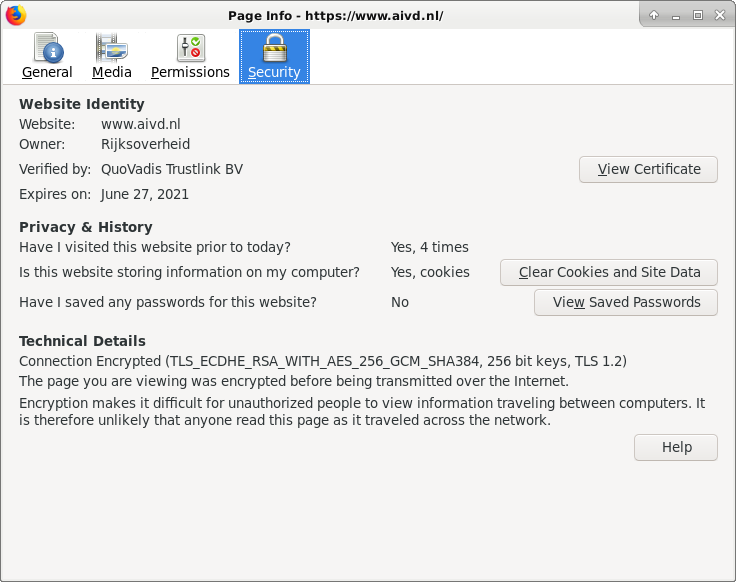
\includegraphics[width=0.9\linewidth]{security_ciphers_aivd.png}
	\caption{Cipher Suite van de AIVD}
	\label{fig:CipherAIVD}
\end{figure}

Bij Technical Details vind je de regel die gaat over de connectie encryptie. Je ziet dat er gekozen is voor TLS 1.2 en 256 bits en dat de cipher suite TLS\_ECHDE\_RSA\_WITH\_AES\_256\_GCM\_SHA384 is. Dat is een hele mondvol, de vraag is wat dit betekent.

\goodbreak
\begin{description}
	\item[TLS] Het TLS protocol waarvan we aan het einde van de regel al gezien hebben dat de keuze gevallen is op TLS versie 1.2
	\item[ECDHE] Het key exchange protocol, Elliptic-Curve Diffie-Hellman Ephemeral.
	\item[RSA] Het encryptie protocol voor de certificaten. De client moet dus RSA gebruiken om de public key te decrypten.
	\item[AES\_256\_GCM] De symmetrische encryptie methode die gebruikt gaat worden voor de encryptie. Alle berichten tussen client en server worden dus versleuteld met 256 bits AES encryptie met Galois/Counter Mode.
	\item[SHA384] Message integrity. Om te controleren dat berichten onderweg niet zijn gewijzigd wordt de SHA functie gebruikt in 384 bits mode.
\end{description}

Het TLS protocol wordt gebruikt (en niet bijvoorbeeld SSL), we gebruiken een vorm van Diffie-Hellman om een symmetrische encryptie sleutel overeen te komen en deze sleutel gebruiken we met AES om alle berichten te encrypten en decrypten. Daarnaast hebben ze besloten om RSA te gebruiken voor de public en private key en worden de berichten gecontroleerd door gebruik te maken van de SHA-hashing techniek. Daarmee hebben we de volledige cipher suite beschreven.

\subsection{Key Exchange}\index{Key exchange}
In het ServerHello bericht hebben we van de server zijn public key gekregen en daarmee kunnen we een encrypted verbinding opzetten tussen de browser en de webserver. Helaas is asymmetrische encryptie erg traag en bij HTTP moeten er heel veel kleine berichten heen en weer gestuurd worden. Het is veel sneller en procesor vriendelijker om AES, een vorm van symmetrische encryptie, te gebruiken. Om over te kunnen stappen van asymmetrisch naar symmetrisch moeten we eerst een gedeelde sleutel met elkaar overeen komen, want alleen met een gedeelde sleutel spreken we van symmetrische encryptie.

Een methode voor het afspreken van een gezamenlijke sleutel moet snel gebeuren, makkelijk schaalbaar zijn en moet over een netwerk gebeuren dat per definitie onbetrouwbaar is..., dat is een behoorlijke uitdaging. We kunnen dus niet zo even over het Internet een sleutel van de een naar de ander sturen en deze gaan gebruiken, want dan kan er altijd iemand die sleutel afluisteren.

De oplossing die gekozen is is het gebruik van een wiskundig grapje dat bedacht is door twee wiskundigen in 1975. Deze wiskundigen zijn Whitfield Diffie en Martin Hellman en de oplossing die zij bedachten heet dan ook Diffie-Hellman\index{Diffie-Hellman}, afgekort DH\index{DH}. Om tot een gezamenlijke sleutel te komen hebben we priemgetallen nodig en een stukje wiskunde dat 'in modulo'-rekenen heet. Dat klinkt moeilijk maar is het niet want je gebruikt het dagelijks zonder dat je erbij nadenkt.

We beginnen met het 'in modulo'-rekenen\index{in modulo}, het staat ook bekend als klok-rekenen\index{klok-rekenen}. Op een analoge klok zijn er 12 uren en die uren komen twee keer per dag langs, 1 keer voor de middag en 1 keer na de middag. Op een digitale klok loopt de klok vaak van 0 tot 24 uur. 13:00 is betekent dan 1 uur in de middag. Wat je doet is 13-12=1 en daardoor weet je dat het 1 uur is. Hetzelfde geldt voor 15:00 uur, dat is 15-12=3 uur in de middag. Voor de uren onder de 12 doe je dit rekensommetje niet. Dit is klokrekenen. 12 is de basis. Als we dit in een wiskundige notatie willen opschrijven dan schrijven we 13mod12 of 15mod12 en spreken dat uit als 13 modulo 12 of 15 modulo 12, daarom heet het in de wiskunde 'in modulo'-rekenen. Op je rekenmachine en in programmeertalen wordt er vaak het procentteken voor gebruikt, dus: 13\%12 of 15\%12.

In modulo rekenen kunnen we natuurlijk ook met andere basis getallen dan 12 doen. 4mod3 is 1. De afspraak bij in modulo rekenen is dat je zovaak het basis getal eraf trekt tot je alleen de rest waarde overhoud. Zo is ook 16mod3 gelijk aan 1, want ik kan 5x het getal 3 van 16 aftrekken en hou dan 1 over.

De andere eis waaraan voldaan moet worden bij DH is dat er gebruik gemaakt moet worden van priemgetallen. Priemgetallen zijn getallen die alleen deelbaar zijn door zichzelf en door 1. Zo is 13 bijvoorbeeld een priemgetal. De enige getallen waardoor 13 deelbaar is is door 13 en door 1.

Als nu twee mensen met elkaar willen communiceren en een gedeelde geheime sleutel willen gebruiken dan kunnen gebruik maken Diffie-Hellman om dat te bereiken. Laten we uit gaan van Alice en Bob die met elkaar berichten willen versturen die met dezelfde sleutel geencrypt zijn.

\begin{flushleft}
\begin{table}[h!]
\centering
	\begin{tabularx}{\textwidth}{ |p{0.3\linewidth}|p{0.3\linewidth}|p{0.3\linewidth}| }
\hline
	Alice &
	Internet &
	Bob\\
\hline
	Alice verzint twee priemgetallen p en g waarbij g kleiner is dan p (p=11, g=7)&
	Alice stuurt p,q naar Bob &
	Bob kent nu p en g\\
\hline
	Alice bedenkt een getal a &
	Dit zijn de private keys en ze gaan niet over het Internet &
	Bob bedenkt een getal b\\
\hline
	$A = g^a mod p$ (A=2)&
	&
	$B = g^b mod p$ (B=4)\\
\hline
	&
	Alice stuurt A naar Bob en Bob stuurt B naar Alice &
	\\
\hline
	$S = B^a mod p$ (S=9)&
	&
	$S = A^b mod p$ (S=9)\\
\hline
\end{tabularx}
\caption{Document wijzigingen}
\label{table:DH}
\end{table}
\end{flushleft}

Over het Internet zijn nu gegaan p, g, A en B. Dus iemand die een aanval op de encryptie wil plegen kent deze getallen, maar dat die aanvaller niet weet zijn de getallen a of b en dus kan de aanvaller nooit S berekenen en omdat het gedeelde geheim S niet over het Internet gegaan is kan de aanvaller S ook niet afluisteren. S is een gedeelde sleutel die door zuiver berekening tot stand is gekomen.

Als we alleen Diffie-Hellman zouden gebruiken dan kunnen we door heel lang monitoren en afluisteren van de verbinding uiteindelijk de sleutel achterhalen omdat altijd dezelde sleutel gebruikt wordt. Dat is niet handig, daarom berekenen systemen regelmatig opnieuw S door hetgeen in tabel \ref{table:DH} staat opnieuw te doen met nieuwe getallen. Het feit dat S maar een korte levensduur heeft noemen in het Engels ephemeral, ofwel kortdurend. Dit noemen we dan ook DHE\index{DHE}\index{Diffie-Hellman Ephemeral}.

De Elliptic-Curve\index{Elliptic-Curve} variant is voornamelijk voor de snelheid.

%\input{src/tls_pfs}
\subsection{Message integrity}\index{Message integrity}\index{MAC}
Nu we alles geencrypt over het Internet kunnen sturen lijkt de wereld veilig, maar die is het nog niet. Neem het volgende scenario:
\begin{lstlisting}
Alice: "Hi Bob, it's Alice. Sent me your key." -> Mallory -> Bob
Alice <- [Mallory's key] <- Mallory <- [Bob's Key] <- Bob
Alice: [EncMallory"Secret message"] -> Mallory: [EncBob"Secret message"] -> Bob
\end{lstlisting}

Wat hier gebeurt is dat Alice om Bob's key vraagt, Mallory vangt dat bericht op en stuurt het door naar Bob. Bob stuurt zijn sleutel naar Alice, maar weer vangt Mallory het bericht op, maar stuurt het nu niet door, maar wijzigt het bericht en vervangt Bob's key met die van haar. Mallory bewaart de sleutel van Bob. Alice denkt dat ze de sleutel van Bob heeft ontvangen en encrypt een geheim bericht met de sleutel die eigenlijk van Mallory is. Mallory vangt het bericht op, decrypt het met het private key, encrypt het met Bob's key en stuurt het bericht door naar Bob. Zowel Alice als Bob denken dat alles goed gegaan is en dat ze een geheim bericht over hebben gestuurd, maar ondertussen heeft Mallory het bericht ook gelezen zonder dat Alice of Bob dat kunnen weten.

Dit probleem moeten we oplossen en dat doen we door gebruik te maken van Message Integrity, bericht integriteit. Het betekent dat we gaan controleren of een bericht dat verstuurt is van Alice naar Bob of van Bob naar Alice onderweg veranderd is, zoals in het bovenstaande gebeurde toen Bob zijn key naar Alice stuurde en Mallory er haar eigen key in stopte.

De eerste stap die we nemen is dat we een hash-waarde berekenen over het bericht, daarvoor gebruiken we SHA384. Die hash is unique dus als we die met het bericht meesturen en de ontvangende kant berekent ook met SHA384 de hash-waarde over het ontvangen bericht en deze waardes zijn hetzelfde dan weten we dat het bericht onderweg niet veranderd is. Behalve als Mallory niet alleen Bob's key vervangt door die van haar, maar ook de SHA384 opnieuw berekent en vervangt, dan zijn we uiteindelijk nog niets opgeschoten.

We moeten er dus voor zorgen dat de hash versleuteld wordt. Voor die versleuteling kunnen we de symmetrische key nemen die we beide al hebben. De zender en ontvanger moeten dus beide een hash berekenen over het bericht en deze hash versleutelen met de symmetrische key. De verzender zendt de uitkomst mee naar de ontvanger en de ontvanger vergelijkt de ontvangen waarde met zijn eigen berekening, als de waardes gelijk zijn weten we zeker dat er onderweg niet geknoeid is met het bericht omdat Mallory nooit de geheime sleutel kan weten. Zo'n versleutelde hash waarde noemen we een MAC, Message Authentication Code.

\subsection{TLS versions}
SSL dient, in welke versie dan ook, niet meer gebruikt te worden omdat er te veel fouten in zitten die door aanvallers misbruikt kunnen worden.

TLS zit inmiddels (2021) in versie 1.3, hoewel versie 1.2 niet volledig veilig is wordt het nog zo algemeen gebruikt dat het niet handig is om TLS 1.2 niet te ondersteunen in de browser. Voor de server ligt dat anders. Alle moderne browsers zoals Firefox, Chrome, Safari, Opera en Edge ondersteunen TLS 1.3, dus het is aan te bevelen om op de server alleen nog TLS 1.3 te ondersteunen. Alleen als je nog oude versies van bepaalde browsers moet ondersteunen kan ook TLS 1.2 ondersteund worden. Alle TLS versies ouder dan 1.2 moeten uit staan, daar deze te veel mogelijkheden bevatten om er misbruik van te maken.

\section{IIS en TLS}\index{IIS}\index{Internet Information Server!TLS}
\subsection{HTTP Strict-Transport-Security (HSTS)}\index{IIS!HSTS}\index{IIS!HTTP Strict-Transport-Security}\index{HSTS!IIS}\index{HTTP Strict-Transport-Security!IIS}
\url{https://www.saotn.org/enable-http-strict-transport-security-hsts-on-iis/}

\subsection{SSL en TLS}\index{IIS!SSL}\index{IIS!TLS}\index{TLS!IIS}\index{SSL!IIS}
Gebruik de registry editor om IIS via SCHANNEL TLS 1.2 of liever nog TLS 1.3 te laten gebruiken dit is een server wide setting, since Windows Server 2019 kan het ook per site (niet behandeld in dit document):
\begin{lstlisting}
HKEY_LOCAL_MACHINE\SYSTEM\CurrentControlSet\Control\SecurityProviders\SCHANNEL\Protocols\TLS 1.2\Server
\end{lstlisting}
zet de DisabledByDefault op 0, zodat het protocol ge-enabled is. Voor de SSL-varianten en voor TLS lager dan 1.2 zet DisabledByDefault op 1 zodat deze varianten gedisabled zijn.

\subsection{Ciphers}\index{IIS!Ciphers}\index{Ciphers!IIS}
De globale, dat is voor alle sites, settings voor ciphers die gebruikt kunnen worden door IIS worden beschreven in de SCHANNEL settings in de registry:
\begin{lstlisting}
[HKEY_LOCAL_MACHINE\SYSTEM\CurrentControlSet\Control\SecurityProviders\Schannel\Ciphers]
[HKEY_LOCAL_MACHINE\SYSTEM\CurrentControlSet\Control\SecurityProviders\Schannel\CipherSuites]
[HKEY_LOCAL_MACHINE\SYSTEM\CurrentControlSet\Control\SecurityProviders\Schannel\Hashes]
[HKEY_LOCAL_MACHINE\SYSTEM\CurrentControlSet\Control\SecurityProviders\Schannel\KeyExchangeAlgorithms]
[HKEY_LOCAL_MACHINE\SYSTEM\CurrentControlSet\Control\SecurityProviders\SCHANNEL\KeyExchangeAlgorithms\Diffie-Hellman]
	"Enabled"=dword:1
	"ServerMinKeyBitLength"=dword:00000800
		1024 bits: 00000400
		2048 bits: 00000800
		4096 bits: 00001000
\end{lstlisting}

\subsection{Hashes}\index{IIS!Hashes}\index{Hashes!IIS}
De globale, dat is voor alle sites, setting voor hashes die gebruikt kunnen worden door IIS worden beschreven in de SCHANNEL settings in de registry:
\begin{lstlisting}
[HKEY_LOCAL_MACHINE\SYSTEM\CurrentControlSet\Control\SecurityProviders\Schannel\Hashes]
\end{lstlisting}

\subsection{Key Exchange}\index{IIS!Key exchange}\index{Key exchange!IIS}
De globale, dat is voor alle sites, setting voor de key exchange die gebruikt kunnen worden door IIS worden beschreven in de SCHANNEL settings in de registry:
\begin{lstlisting}
[HKEY_LOCAL_MACHINE\SYSTEM\CurrentControlSet\Control\SecurityProviders\Schannel\KeyExchangeAlgorithms]
[HKEY_LOCAL_MACHINE\SYSTEM\CurrentControlSet\Control\SecurityProviders\SCHANNEL\KeyExchangeAlgorithms\Diffie-Hellman]
	"Enabled"=dword:1
	"ServerMinKeyBitLength"=dword:00000800
		1024 bits: 00000400
		2048 bits: 00000800
		4096 bits: 00001000
\end{lstlisting}


\chapter{Network Attacks}
\section{DoS}\index{DoS}\index{Denial of Service}
Een Denial of Service attack zorgt ervoor dat een bepaalde dienst niet bereikbaar is. Er zijn verschillende technieken om dit te bereiken:
\begin{itemize}
\item Heel veel data versturen naar een systeem waardoor alle bandbreedte wordt gebruikt
\item Heel veel requests naar een service sturen waardoor de service zo druk is dat er geen nieuwe service requests aangenomen kunnen worden
\item Een machine op een andere manier overbelasten waardoor deze uiteindelijk niet meer kan functioneren
\end{itemize}

Een aanvaller met een grotere bandbreedte dan een server kan makkelijk de lijn van de server volspoelen, zodat deze verder geen data meer kan ontvangen. Dit was een techniek die in het verleden beter werkte dan tegenwoordig. De meeste thuisgebruikers hebben tegenwoordig een fractie van de bandbreedte die een gemiddeld bedrijf geeft voor zijn Internet verbinding.

Als je weet wat het operating systeem is van de aan te vallen server, dan kan je opzoeken wat het maximum aantal requests is wat een dienst kan ondersteunen. Als jij instaat bent om meer dan deze hoeveelheid requests naar een dienst kan sturen dan kan je ervoor zorgen dat de dienst niet meer beschikbaar is.

Andere mogelijkheden om servers plat te laten is bijvoorbeeld door te zorgen dat er niet voldoende diskruimte meer is. Ook dit is een vorm van een Denial of Service attack. Een van de mogelijkheden die je als aanvaller hebt is door bijvoorbeeld zoveel logging te veroorzaken dat een server op een geven moment andere data niet meer kwijt kan op de disk.

De makkelijkste manier om een Denial of Service attack af te slaan is door je provider te vragen het IP-adres van de aanvaller te blokkeren. Het mooist is natuurlijk als je de provider van de aanvaller kan vragen om de verbinding van de aanvaller te verbreken of te blokkeren. Een andere maatregel is het beperken van het maximum aantal connecties dat een enkele source mag opzetten.

\subsection{DDoS}\index{DDoS}\index{Distributed Denial of Service}
Een Distributed Denial of Service attack is een DOS die uitgevoerd wordt door gebruik te maken van meerdere systemen op het Internet. Door meerdere systemen te gebruiken kan de aangevallen server niet beschermd worden door \'e\'en IP-adres te blokkeren. Het feit dat de aanval van verschillende IP-adressen komt maakt het vele malen moeilijker om deze aanval af te slaan. Een DDoS wordt dus uitgevoerd door verschillende machines een aanval te laten uitvoeren op een enkele host of dienst. Een aanvaller stuurt hiervoor een zogenaamde Command \& Control-server aan die op zijn beurt de verschillende machines in een Bot-net\index{Bot-net} aanstuurt.

Er zijn twee soorten aanvallen, de aanvallen op netwerkniveau en de aanvallen op applicatieniveau.

De aanvallen op de netwerk-layers (OSI layers 3 en 4) bestaan uit SYN, UDP of ICMP-floods of reflection attacks (DNS, NTP). Deze aanvallen zijn gericht op de bandbreedte en de servercapaciteit. De tegen maatregelen bestaan uit het uitfilteren van de juiste packetten, zorgen dat je voldoende extra bandbreedte beschikbaar hebt, gebruik van DNS uitwijk mogelijkheden, loadbalancers en het in voorraad hebben van extra servercapaciteit.

De aanvallen op applicatieniveau zijn complexer en komen daardoor minder vaak voor. Het belangrijkste wapen tegen deze aanvallen is de WAF\index{WAF} (Web Application Firewall\index{Web Application Firewall}).

\section{Gaining access}
Door gebruik te maken van fouten (bugs) in de server, scriptingtaal of in de beveiliging van de database kan een aanvaller toegang krijgen tot het onderliggende bestandssysteem, tot de database of zelfs tot de gehele server.

\subsection{Defacing}\index{Deface}
Als een aanvaller toegang heeft gekregen tot de inhoud van de database achter de website of data kan schrijven naar de disks waarop de website staat dan kan de aanvaller de inhoud van de pagina's wijzigen. In de begin dagen werden websites 'defaced', wat betekent dat de aanvaller de bestaande webpagina verving met zijn eigen ontworpen pagina, meestal met de mededeling wie de 'deface' had gedaan. Het ging om de eer, om te laten zien dat iemand het kon. Natuurlijk leverde dit imago schade op voor het bedrijf waarvan de pagina gedefaced was, maar er werd verder meestal geen schade aangebracht.

\subsection{Server access}
Via een fout in bijvoorbeeld de code van de webserver of een scriptingtaal zou een aanvaller toegang kunnen krijgen tot de server (shell-access), of via een bug data kunnen schrijven naar het bestandssysteem.

Als de aanvaller via een bug data kan schrijven naar het bestandssysteem, dan zou deze ook bestaande bestanden kunnen overschrijven, afhankelijk van hoe de rechten op het systeem zijn ingesteld. Het is dus van belang om de webserver de meest minimale rechten te geven op de bestanden waar het proces bij moet kunnen, meestal betekent dat dat read-only rechten voldoende zijn. Het server-proces hoeft geen data te kunnen schrijven. Een aparte gebruiker kan dan de rechten krijgen om de bestanden op de server aan te passen.

Ook als een aanvaller shell-access of executie-rechten kan krijgen via de server is het van belang dat de rechten (gebruiker) waaronder de server-draait de minst mogelijke rechten heeft.

\subsubsection{IIS owner and rights}\index{IIS!Owner}\index{IIS!Rights}
Microsoft heeft een uitgebreid document geschreven over de users en groepen die gebruikt worden door IIS: \url{https://docs.microsoft.com/en-us/troubleshoot/iis/default-permissions-user-rights}

\subsection{Database access}
Database\index{database} access betekent dat de aanvaller data in de database die achter de website zit kan wijzigen. Hiermee kan de aanvaller dus zorgen dat de inhoud van een webpagina verandert, of erger hij kan de totale klantendatabase lezen, al dan niet met wachtwoorden, rekeningnummers, etc.


\chapter{Webserver Attacks}\index{Webserver attacks}
\section{Slowloris}\index{Slowloris}
HTTP is ontworpen om te kunnen werken over goeie en slechte netwerken verbindingen (snel en langzaam), HTTP zal proberen om een goed HTTP pakket dat binnenkomt te behandelen en er antwoord op te geven. HTTP is dus heel geduldig als er data binnenkomt, als er maar elke keer wat binnen komt dan houdt HTTP de verbinding open. Slowloris maakt hier misbruik van door een well-formed HTTP request \'e\'en character per keer te sturen. Door goed gekozen pauzes te kiezen tussen de characters, zodat er net geen time-out ontstaat, kan een verbinding voor minuten open gehouden worden en is deze verbinding dus niet beschikbaar voor nieuwe connecties. Ook een niet compleet request kan de lijn open houden. Als je voldoende van deze lijnen opzet kan een server op een gegeven moment geen nieuwe verbindingen meer aannemen.

Een manier om slowloris te voorkomen is het zetten een timeout die de verbinding afbreekt als het langer duurt dan bijvoorbeeld 60 seconden om een request binnen te krijgen.


\subsection{IIS en slowloris}\index{Slowloris!IIS}\index{IIS!Slowloris}
Voor versies van IIS 7 tot IIS 10 kun je op de volgende manier de time-out settings wijzigen:
\begin{enumerate}
\item Ga op de server naar het Control Panel, selecteer de Administrative Toole en selecteer Internet Information Services (IIS) Manager.
\item Expand the local computer node, expand "Web Sites", right-click op de website waar het om gaat website en bij "Manage Web Site" selecteer de Advanced Settings.
\item In het Advanced Settings window, expand Connection Limits, bij het "Connection time-out" veld kan je de waarde wijzigen en daarna op OK klikken.
\end{enumerate}

\section{Cross-Side Request Forgery}\index{CSRF}\index{Cross-Side Request Forgery}
Cross-Site Request Forgery is een exploit methode die het vertrouwen van de site in de user (user browser) misbruikt. De aanval probeert ervoor te zorgen dat een gebruiker iets naar een website stuurt wat niet de bedoeling is. Een aanvaller zou bijvoorbeeld in een post op een forum een bericht kunnen achterlaten met daarin de HTML-tag:
\begin{lstlisting}
<img src="https://stemopmij.nl/dennisisthebest.html">
\end{lstlisting}
Omdat een image geen click behoeft om aangesproken te worden, maar door een browser altijd geladen wordt wordt de opgenomen URL meteen uitgevoerd. Op deze manier kan je valse stemmen genereren.

\section{Cross-Side Scripting}\index{XSS}\index{Cross-Side Scripting}
Cross-Site Scripting (XSS) maakt misbruik van het vertrouwen dat een gebruiker heeft in de website die hij of zij benadert. Als een aanvaller in een bericht op bijvoorbeeld een forum extra code in zijn bericht kan zetten dan zal elke browser die het bericht leest deze client-side code vertrouwen omdat hij van een "vertrouwde" site komt. Op deze manier kan een aanvaller toegang krijgen tot session-keys, cookies of andere site-informatie die is opgeslagen op de client. De bouwer van een website moet dan ook zorgen dat dit soort code niet ge\"injecteerd kan worden.

Volgens de Mozilla website\footnote{https://developer.mozilla.org/en-US/docs/Web/Security/Types\_of\_attacks} kunnen we 3 soorten XSS-aanvallen onderscheiden:
\begin{description}
	\item[Stored XSS Attacks]\index{Stored XSS Attacks}\index{XSS!Stored XSS Attacks} Waarbij de malicious-code opgeslagen is op de server die de client bezoekt
	\item[Reflected XSS Attacks]\index{Reflected XSS Attacks}\index{XSS!Reflected XSS Attacks} Hierbij staat de malicious-code niet op de server, maar komt deze via een omweg, bijvoorbeeld een zou resultaat of een error message bij de browser terecht. De code wordt dan dus doorgegeven door de server zonder dat deze het weet en voor de browser lijkt de data van de server te komen.
	\item[DOM-based XSS Attacks]\index{DOM-based XSS Attacks}\index{XSS!DOM-based XSS Attacks} De DOM is de omgeving waarin een pagina "leeft". Met JavaScript kan je bijvoorbeeld een pagina on-the-fly wijzigen, dat doe je door de DOM te manipuleren. Dit kan ook misbruikt worden via een XSS-aanval.
\end{description}

Headers die gezet moeten worden vanuit de web-applicatie\index{X-XSS-Prection}\index{Header!X-XSS-Protection}:
\begin{lstlisting}
X-XSS-Protection: 1; mode=block
\end{lstlisting}

Een bredere beveiliging tegen XSS is zijn CSP (Content Security Policy) headers, die beperken waar een bepaald object vandaan mag komen\index{default-src}\index{script-src}\index{img-src}\index{child-src}\index{Content-Security-Policy!default-src}\index{Content-Security-Policy!script-src}\index{Content-Security-Policy!img-src}\index{Content-Security-Policy!child-src}\index{insafe-inline}.
\begin{lstlisting}
Content-Security-Policy: default-src 'self'; script-src 'self' 'unsafe-inline'; img-src 'https://*'; child-src 'none';
\end{lstlisting}
Je mag een Content-Security-Policy ook meegeven via de META data van een HTML pagina:
\begin{lstlisting}
<meta http-equiv="Content-Security-Policy"
      content="default-src 'self'; img-src https://*; child-src 'none';">
\end{lstlisting}

Voor een compleet overzicht van CSP zie de website \url{https://content-security-policy.com/}.

Stel dat we een website beheren die als header meegeeft naar de browser: Content-Security-Policy script-src 'https://example.com'. Dan kunnen scripts alleen vanaf domein afkomstig zijn. Inline JavaScript gaat dus niet werken. Er is echter een truc om hier omheen te werken, die maakt gebruikt van MIME-sniffing.

Het Internet is gemaakt om tekst in de ASCII\footnote{American Standard Code for Information Interchange: een encoding standaard om tekst om te zetten naar getallen, zodat een computer er mee kan werken en zodat tekst getransporteerd kan worden via digitale media} character set te versturen, binaire data kunnen we niet zo versturen. Binaire data moet eerst omgezet worden in de characters die in de ASCII tabel voorkomen. Deze omzetting wordt gedaan door gebruik te maken van MIME (Multipurpose Internet Mail Extension), zoals de naam duidelijk maakt ooit bedacht voor mail, nu ook gebruikt voor veel meer zaken, onder andere voor HTTP. Als data verstuurd wordt over het Internet dat kan de Content-Type\index{Content-Type}\index{Header!Content-Type} header gebruikt worden om aan te geven dat data bijvoorbeeld een HTML-pagina is door de MIME-type te zetten naar text/HTML. Echter als de Content-Type header niet aanwezig is dan zal een browser op best-effort basis proberen uit te zoeken wat voor type data het heeft binnen gekregen. Dit naar beste kunnen interpreteren van binnengekomen data heet MIME-sniffing. Het kan ook gebeuren dat een programmeur bijvoorbeeld een foutje heeft gemaakt en dat de Content-Type op text/plain staat, maar dat de browser ontdekt dat het eigenlijk JavaScript is. Zonder veel omhaal zullen de meeste browser de code dan uitvoeren in de veronderstelling dat dat eigenlijk is wat de gebruiker wil. Deze "feature" die het voor de gebruiker makkelijker moet maken opent ook een gat in de veiligheid.

Als een aanvaller de kans heeft om een tekst bestand op de server te zetten met daarin JavaScript code dan kan hij doormiddel van een HTML-tag zoals:
\begin{lstlisting}
<script src="https://example.com/hack.txt"></script>
\end{lstlisting}
de code bij de browser krijgen. De Content-Type header zal keurig text/plain melden en de browser zal ontdekken dat er JavaScript aangeboden wordt en deze uitvoeren. Om dit uitvoeren te voorkomen moet er een andere header gezet worden\index{X-Content-Type-Options}\index{Header!X-Content-Type-Options}\index{nosniff}:
\begin{lstlisting}
X-Content-Type-Options: nosniff
\end{lstlisting}
Deze optie vertelt de browser dat hij de Content-Type header serieus moet nemen en niet zijn eigen interpretatie erop los mag laten. Let echter wel op! als de Content-Type text/plain is en de X-Content-Type-Options is op nosniff gezet dan zal de browser letterlijk doen wat je wil en de tekst weergeven als plain tekst. Als het dus code of een HTML pagina was dan ziet de gebruiker de broncode, het is dus cruciaal dat de Content-Type header goed staat.

\subsection{XSS en PHP}
Als je op een website een formulier hebt dat er ongeveer zo uit ziet:
\begin{lstlisting}
<form action="myform.php" method="post">
 <input type="text" name="textfield" value="">
 <input type="submit" name="submit" value="Submit">
</form>
\end{lstlisting}

En een aanvaller vult in het textfield geen gewone tekst in maak bijvoorbeeld een stukje JavaScript:
\begin{lstlisting}
<script>alert("Hello world!")</script>
\end{lstlisting}

dan wordt de JavaScript code uitgevoerd door de browser als je de data zonder verdere controle afbeeld via echo:
\begin{lstlisting}
echo $_POST["textfield"];
\end{lstlisting}

Dit kan je tegen gaan door bijvoorbeeld JavaScript alleen toe te staan als het script geladen wordt als extern script van het eigen domein\index{script-src}, inline JavaScript is dan automatisch verboden:
\begin{lstlisting}
script-src 'self'
\end{lstlisting}

\subsection{XSS en Cookies}
Als je gebruik maakt van cookies dan kan je met een additionele header voorkomen dat client-side scripts bij de cookie kunnen (als de browser de header ondersteunt). De extra header heet HttpOnly\index{Set-Cookie!HttpOnly} en wordt gebruikt in de Set-Cookie header:

\begin{lstlisting}
Set-Cookie ^(.*)$ $1;HttpOnly;Secure
\end{lstlisting}
Als de HttpOnly optie gezet is bij de Set-Cookie header, dan mag geen enkel Client-Side script bij de cookie komen.

Voor meer informatie over Set-Cookie zie de website van Mozilla: \url{https://developer.mozilla.org/en-US/docs/Web/HTTP/Headers/Set-Cookie}



%%%%%%%%%%%%%%%%%%%%%
%%% Index and End %%%
%%%%%%%%%%%%%%%%%%%%%
%\backmatter
\printindex
\end{document}

%%% Last line %%%
